\documentclass[12pt]{article}

\usepackage{sbc-template}
\usepackage{graphicx,url}
\usepackage[utf8]{inputenc}
\usepackage[brazil]{babel}

     
\sloppy

\title{Monolito e Microsserviços para Iniciantes: Um Comparativo Prático}

\author{Davi G. Nascimento\inst{1}, João V. Sales\inst{1}, Pedro Faria Barreto\inst{1}, Pedro H. Poderoso\inst{1} }


\address{Universidade Tiradentes (UNIT-SE)\\
  Aracaju -- SE -- Brazil
}

\begin{document} 

\maketitle

\begin{abstract}
  This meta-paper describes the style to be used in articles and short papers
  for SBC conferences. For papers in English, you should add just an abstract
  while for the papers in Portuguese, we also ask for an abstract in
  Portuguese (``resumo''). In both cases, abstracts should not have more than
  10 lines and must be in the first page of the paper.
\end{abstract}
     
\begin{resumo} 
  Este meta-artigo descreve o estilo a ser usado na confecção de artigos e
  resumos de artigos para publicação nos anais das conferências organizadas
  pela SBC. É solicitada a escrita de resumo e abstract apenas para os artigos
  escritos em português. Artigos em inglês deverão apresentar apenas abstract.
  Nos dois casos, o autor deve tomar cuidado para que o resumo (e o abstract)
  não ultrapassem 10 linhas cada, sendo que ambos devem estar na primeira
  página do artigo.
\end{resumo}


\section{Introdução}

Ao dar os primeiros passos no desenvolvimento de software, é natural concentrar os estudos em atividades práticas, como aprender a sintaxe de uma linguagem de programação, elaborar algoritmos, conectar uma aplicação a um banco de dados e criar interfaces interativas. Além dessas atividades, é necessário pensar em como organizar os componentes de um sistema para que ele atenda às suas necessidades de desempenho, segurança e manutenção, tanto no início de seu desenvolvimento quanto à medida que evolui, para garantir um desenvolvimento consistente.

\subsection{A necessidade de uma arquitetura de software}

De forma geral, a arquitetura de software pode ser entendida como o conjunto de estruturas necessárias para raciocinar sobre um sistema, compreendendo seus elementos, as relações entre eles e as propriedades de ambos \cite{bass:2013}. Uma visão complementar considera que a arquitetura reúne as decisões de projeto mais importantes de um sistema, isto é, aquelas que, uma vez tomadas, dificilmente poderão ser revertidas, como a divisão do sistema em módulos e a escolha da linguagem de programação e do banco de dados \cite{valente:2020}. Atributos de qualidade como desempenho, segurança, disponibilidade e facilidade de manutenção não surgem espontaneamente: eles são habilitados ou limitados por essas decisões, geralmente tomadas no início do projeto \cite{bass:2013,cintra:2025}. Todo sistema possui uma arquitetura, mesmo que ela não tenha sido conscientemente projetada; no entanto, nem toda arquitetura é adequada aos objetivos do sistema \cite{bass:2013}.

A necessidade de uma arquitetura bem definida, contudo, manifesta-se de forma diferente conforme o ambiente em que o software é desenvolvido. Em projetos pequenos, como trabalhos acadêmicos, protótipos e produtos de empresas em estágio inicial, a prioridade costuma ser entregar funcionalidades rapidamente com uma equipe reduzida; nesse cenário, uma arquitetura simples, fácil de desenvolver, testar e implantar, tende a ser a mais vantajosa \cite{ciriano:2025}. Em organizações maiores, com vários times trabalhando sobre o mesmo produto, a arquitetura passa a ser também um instrumento de coordenação, pois define as fronteiras e as interfaces entre as partes do sistema e permite que cada time evolua a sua parte com menos interferência dos demais. Não por acaso, a Lei de Conway afirma que as organizações tendem a produzir sistemas cuja estrutura reflete a sua própria estrutura de comunicação \cite{conway:1968,valente:2020}. Já em sistemas expostos a grandes volumes de acesso, como lojas virtuais e plataformas de \textit{streaming}, a arquitetura precisa garantir escalabilidade e disponibilidade, de modo que um pico de uso ou a falha de um componente não interrompa todo o serviço \cite{newman:2015}. Por fim, em sistemas de longa duração, a ausência de uma organização clara favorece a chamada erosão arquitetural: alterações sucessivas que violam a estrutura original tornam o software cada vez mais frágil e custoso de manter \cite{perry:1992}.

Um episódio histórico ilustra como as decisões arquiteturais podem levar anos para revelar suas consequências. Em 1992, Andrew Tanenbaum e Linus Torvalds debateram publicamente a arquitetura do recém-criado Linux, que seguia um modelo monolítico, no qual todas as funções do sistema operacional são implementadas em um único executável. Tanenbaum defendia uma arquitetura de \textit{microkernel}, em que apenas as funções mais básicas permanecem no núcleo e as demais são executadas como processos independentes. Quase duas décadas depois, o próprio Torvalds reconheceu que o \textit{kernel} havia se tornado grande e inchado, e que cada nova funcionalidade piorava esse cenário \cite{valente:2020}.

\subsection{Monolito e microsserviços}

Entre as diversas formas de organizar um sistema, duas abordagens se destacam atualmente: a arquitetura monolítica e a arquitetura de microsserviços \cite{borges:2025}. Na arquitetura monolítica, ilustrada na Figura~\ref{fig:monolito}, todas as funcionalidades da aplicação (interface, regras de negócio e acesso a dados) são desenvolvidas, testadas e implantadas como uma única unidade \cite{ciriano:2025}. Isso não significa que o código esteja desorganizado: um monolito pode, e deve, ser dividido internamente em módulos bem definidos. O que o caracteriza é o seu comportamento em tempo de execução, já que todos os módulos são executados pelo sistema operacional como um único processo, compartilhando o mesmo espaço de memória e, normalmente, o mesmo banco de dados \cite{valente:2020}. Dessa forma, a comunicação entre os módulos ocorre por meio de simples chamadas de função, com latência mínima, e operações que envolvem vários módulos podem ser protegidas por uma única transação no banco de dados. Por outro lado, qualquer alteração, por menor que seja, exige gerar e implantar novamente a aplicação inteira; e, quando apenas uma funcionalidade enfrenta alta demanda, a única forma de escalar o sistema é replicá-lo por completo \cite{ciriano:2025}.


\begin{figure}[ht]
\centering
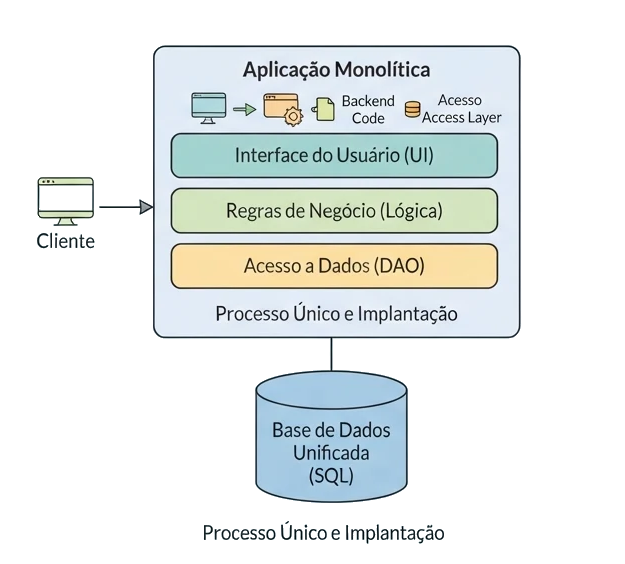
\includegraphics[width=.6\textwidth]{figuras/monolito.png}
\caption{Arquitetura monolítica: os módulos da aplicação são executados em um único processo e compartilham o mesmo banco de dados.}
\label{fig:monolito}
\end{figure}

Na arquitetura de microsserviços, ilustrada na Figura~\ref{fig:microsservicos}, o sistema é decomposto em serviços pequenos e autônomos, cada um responsável por uma capacidade específica do negócio, executado em seu próprio processo e implantado de forma independente dos demais \cite{lewis:2014,newman:2015}. A divisão em módulos, portanto, deixa de existir apenas no código-fonte e passa a existir também em tempo de execução \cite{valente:2020}. Como um serviço não consegue mais acessar variáveis ou estruturas internas de outro, toda a comunicação ocorre por meio de interfaces públicas e através da rede, seja de forma síncrona, por APIs HTTP/REST ou gRPC, seja de forma assíncrona, por filas de mensagens \cite{ciriano:2025}. Idealmente, cada microsserviço também gerencia os próprios dados, em um banco de dados que não é compartilhado com os demais serviços \cite{valente:2020}.


\begin{figure}[ht]
\centering
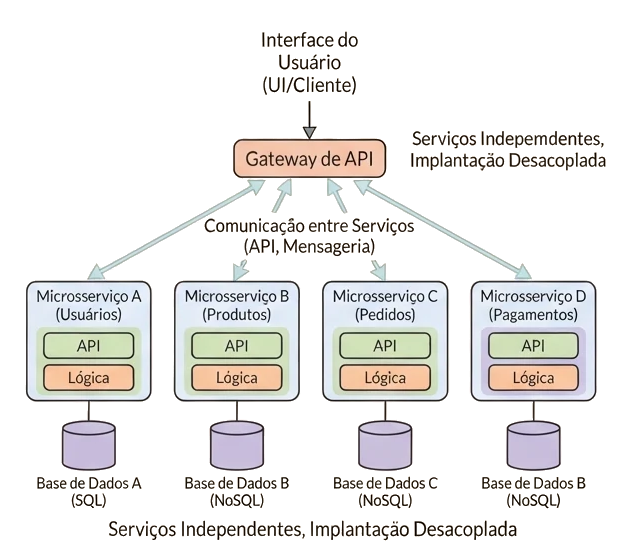
\includegraphics[width=.8\textwidth]{figuras/microsservicos.png}
\caption{Arquitetura de microsserviços: cada serviço é executado em um processo próprio, possui o seu banco de dados e se comunica com os demais pela rede.}
\label{fig:microsservicos}
\end{figure}

Essa diferença técnica traz consequências práticas nos dois sentidos. Os microsserviços permitem escalar apenas os serviços mais demandados, adotar tecnologias diferentes em cada serviço e isolar falhas, de modo que a indisponibilidade de um serviço não precisa derrubar todo o sistema \cite{valente:2020,newman:2015}. Em contrapartida, por construção, eles dão origem a um sistema distribuído e herdam os seus desafios: chamadas pela rede são mais lentas e podem falhar, operações que alteram dados em mais de um serviço deixam de contar com uma transação única, e a implantação, o monitoramento e a depuração passam a envolver diversos processos e ferramentas adicionais \cite{valente:2020,ciriano:2025}. Entre os dois extremos existe ainda o monolito modular, que mantém uma única unidade de implantação, mas impõe fronteiras rígidas entre os módulos, o que pode facilitar uma futura migração \cite{cintra:2025}.

\subsection{Por que surgiram os microsserviços}

Durante muitos anos, a arquitetura monolítica foi o modelo predominante, em razão de sua simplicidade e coesão \cite{morais:2025}. À medida que os sistemas e as equipes cresceram, porém, suas limitações tornaram-se evidentes. Com a adoção de métodos ágeis, o desenvolvimento passou a ser iterativo, com a expectativa de entregas frequentes. Em um monolito, entretanto, uma mudança feita por um time em um módulo pode causar efeitos colaterais em módulos mantidos por outros times. Para evitar que esses erros chegassem aos usuários, as empresas adotavam processos de liberação de versões rigorosos e burocráticos, o que criava um gargalo: o desenvolvimento havia se tornado ágil, mas a entrada em produção continuava lenta \cite{valente:2020}.

A ideia de dividir sistemas em serviços independentes não é inteiramente nova. A Arquitetura Orientada a Serviços (SOA, do inglês \textit{Service-Oriented Architecture}) já propunha construir e integrar aplicações por meio da composição de serviços distribuídos e fracamente acoplados \cite{azevedo:2020}. Os microsserviços são vistos na literatura ora como uma evolução, ora como uma forma particular de implementar a SOA \cite{azevedo:2020,lucio:2017}, diferenciando-se pela ênfase em serviços menores, implantação independente e automatizada, gestão descentralizada de tecnologias e de dados e comunicação por mecanismos leves \cite{lewis:2014}. O termo \textit{microservices} foi discutido em um encontro de arquitetos de software próximo a Veneza, em 2011, adotado pelo mesmo grupo em 2012 e popularizado em 2014 por \cite{lewis:2014}, que sistematizaram as características comuns desse estilo. No mesmo período, empresas como Netflix e Amazon passaram a relatar ganhos significativos ao dividir suas aplicações monolíticas em serviços menores e independentes \cite{newman:2015,cintra:2025}.

A adoção desse estilo só se tornou viável com a evolução da infraestrutura. Plataformas de computação em nuvem permitiram alugar máquinas virtuais sob demanda, tornando simples acrescentar novas instâncias de um serviço \cite{valente:2020}; os contêineres, popularizados pelo Docker em 2013, passaram a empacotar cada serviço com suas dependências de forma leve e portável; e orquestradores como o Kubernetes, lançado pelo Google em 2014, automatizaram a gestão desses contêineres em larga escala \cite{silva:2023}. Somam-se a isso as práticas de DevOps e de integração e entrega contínuas, que automatizam a construção, o teste e a implantação de cada serviço \cite{ciriano:2025}. Ainda assim, a adoção de microsserviços exige maturidade técnica e organizacional \cite{ciriano:2025}. O próprio Fowler observa que quase todos os casos bem-sucedidos começaram com um monolito que cresceu demais e foi dividido, enquanto sistemas construídos como microsserviços desde o início frequentemente enfrentaram sérios problemas \cite{fowler:2015}.

\subsection{Objetivo do trabalho}

Diante desse cenário, nenhuma das duas abordagens é universalmente superior: cada uma apresenta características, vantagens e limitações que devem ser consideradas de acordo com os requisitos do projeto, a experiência da equipe e os recursos disponíveis \cite{borges:2025}. Para quem está iniciando no desenvolvimento de software, porém, essas diferenças costumam ser apresentadas apenas de forma conceitual, o que dificulta perceber o seu impacto concreto.

Este artigo tem como objetivo apresentar e comparar as arquiteturas monolítica e de microsserviços de forma introdutória e prática. Para isso, uma mesma aplicação de agendamento para uma barbearia foi desenvolvida nas duas arquiteturas, atendendo aos mesmos requisitos, expondo a mesma interface HTTP e utilizando a mesma pilha de tecnologias, de modo que apenas a arquitetura varie entre as implementações. A comparação é realizada por meio de uma mesma suíte de testes de aceitação e de \textit{benchmarks} executados sobre as duas versões, buscando identificar as diferenças práticas entre elas e contribuir para a compreensão dos fatores envolvidos na escolha de uma arquitetura.

\section{General Information}

All full papers and posters (short papers) submitted to some SBC conference,
including any supporting documents, should be written in English or in
Portuguese. The format paper should be A4 with single column, 3.5 cm for upper
margin, 2.5 cm for bottom margin and 3.0 cm for lateral margins, without
headers or footers. The main font must be Times, 12 point nominal size, with 6
points of space before each paragraph. Page numbers must be suppressed.

Full papers must respect the page limits defined by the conference.
Conferences that publish just abstracts ask for \textbf{one}-page texts.

\section{First Page} \label{sec:firstpage}

The first page must display the paper title, the name and address of the
authors, the abstract in English and ``resumo'' in Portuguese (``resumos'' are
required only for papers written in Portuguese). The title must be centered
over the whole page, in 16 point boldface font and with 12 points of space
before itself. Author names must be centered in 12 point font, bold, all of
them disposed in the same line, separated by commas and with 12 points of
space after the title. Addresses must be centered in 12 point font, also with
12 points of space after the authors' names. E-mail addresses should be
written using font Courier New, 10 point nominal size, with 6 points of space
before and 6 points of space after.

The abstract and ``resumo'' (if is the case) must be in 12 point Times font,
indented 0.8cm on both sides. The word \textbf{Abstract} and \textbf{Resumo},
should be written in boldface and must precede the text.

\section{CD-ROMs and Printed Proceedings}

In some conferences, the papers are published on CD-ROM while only the
abstract is published in the printed Proceedings. In this case, authors are
invited to prepare two final versions of the paper. One, complete, to be
published on the CD and the other, containing only the first page, with
abstract and ``resumo'' (for papers in Portuguese).

\section{Sections and Paragraphs}

Section titles must be in boldface, 13pt, flush left. There should be an extra
12 pt of space before each title. Section numbering is optional. The first
paragraph of each section should not be indented, while the first lines of
subsequent paragraphs should be indented by 1.27 cm.

\subsection{Subsections}

The subsection titles must be in boldface, 12pt, flush left.

\section{Figures and Captions}\label{sec:figs}


Figure and table captions should be centered if less than one line
(Figure~\ref{fig:exampleFig1}), otherwise justified and indented by 0.8cm on
both margins, as shown in Figure~\ref{fig:exampleFig2}. The caption font must
be Helvetica, 10 point, boldface, with 6 points of space before and after each
caption.

\begin{figure}[ht]
\centering
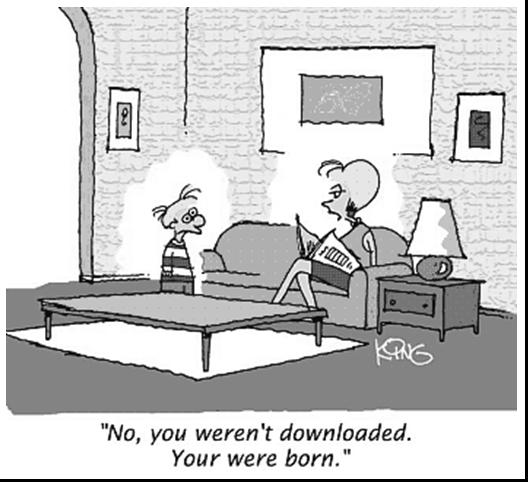
\includegraphics[width=.5\textwidth]{figuras/fig1.jpg}
\caption{A typical figure}
\label{fig:exampleFig1}
\end{figure}

\begin{figure}[ht]
\centering
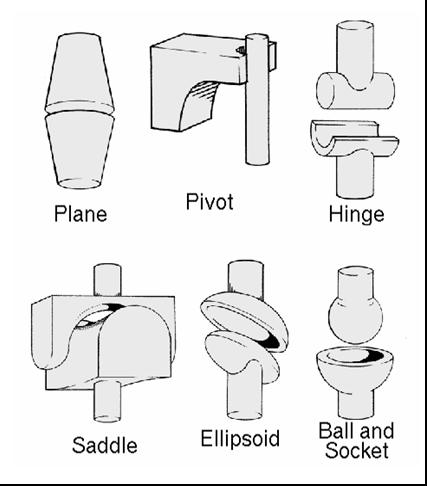
\includegraphics[width=.3\textwidth]{figuras/fig2.jpg}
\caption{This figure is an example of a figure caption taking more than one
  line and justified considering margins mentioned in Section~\ref{sec:figs}.}
\label{fig:exampleFig2}
\end{figure}

In tables, try to avoid the use of colored or shaded backgrounds, and avoid
thick, doubled, or unnecessary framing lines. When reporting empirical data,
do not use more decimal digits than warranted by their precision and
reproducibility. Table caption must be placed before the table (see Table 1)
and the font used must also be Helvetica, 10 point, boldface, with 6 points of
space before and after each caption.

\begin{table}[ht]
\centering
\caption{Variables to be considered on the evaluation of interaction
  techniques}
\label{tab:exTable1}
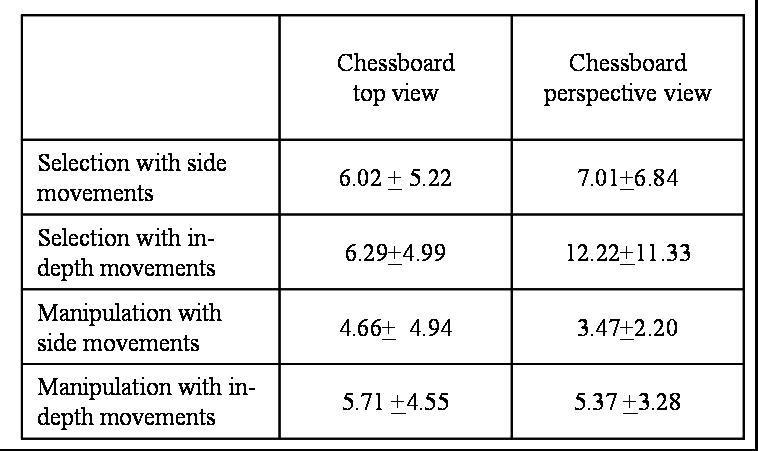
\includegraphics[width=.7\textwidth]{figuras/table.jpg}
\end{table}

\section{Images}

All images and illustrations should be in black-and-white, or gray tones,
excepting for the papers that will be electronically available (on CD-ROMs,
internet, etc.). The image resolution on paper should be about 600 dpi for
black-and-white images, and 150-300 dpi for grayscale images.  Do not include
images with excessive resolution, as they may take hours to print, without any
visible difference in the result. 

\section{References}

Bibliographic references must be unambiguous and uniform.  We recommend giving
the author names references in brackets, e.g. \cite{knuth:84},
\cite{boulic:91}, and \cite{smith:99}.

The references must be listed using 12 point font size, with 6 points of space
before each reference. The first line of each reference should not be
indented, while the subsequent should be indented by 0.5 cm.

\bibliographystyle{sbc}
\bibliography{sbc-template}

\end{document}
